\documentclass[11pt,a4paper]{article}

\usepackage[polish]{babel}
\usepackage[utf8]{inputenc}
\usepackage{polski}
\usepackage[T1]{fontenc}
\usepackage{indentfirst}
\usepackage{wrapfig}    % for wrapping figures, tables
\usepackage{isotope}
\usepackage{hyperref}
\usepackage{amsmath}
\usepackage{amssymb}
\usepackage{bm}
\usepackage{gensymb}
\usepackage{epsfig}
\usepackage{graphics}
\usepackage[shortlabels]{enumitem}
\usepackage{xspace}
\xspaceaddexceptions{[]\{\}}

%\def\hidesolutions{}  %← show solutions. Comment out to show solutions

%
%
%fixpagesize
\pagestyle{empty}
\addtolength{\textwidth}{4cm}
\addtolength{\textheight}{6cm}
\addtolength{\evensidemargin}{-3cm}
\addtolength{\oddsidemargin}{-2cm}
\addtolength{\topmargin}{-3cm}
\parindent=0cm

%
%
% Changes figure placing algorithm
\renewcommand{\topfraction}{1}       % maximal fraction of a page allowed for figures
\renewcommand{\textfraction}{0.15}   % minimal number of text for figure-text shared pages
\renewcommand{\floatpagefraction}{0.95} % if two above does not help, this could do the job 
                                        % must be: floatpagefraction < topfraction !!!!
\renewcommand{\textfraction}{0} % minimum fraction of page, which must be  devoted to text
\renewcommand{\topfraction}{1}  % maximum fraction at top, which can be occupied whit floats
\setcounter{totalnumber}{400}   % increase the number of floats for one page
\setcounter{topnumber}{200}     % at all/top/bottom.
\setcounter{bottomnumber}{200}  %

%
%
%small distance in list/item/enum for enumitem package
\setlist[itemize,enumerate]{topsep=0em}
\setlist{noitemsep}

%Nuclear notations: usage \nucl{235}{92}{U}. Math mode optional
\newcommand{\nucl}[3]{\ensuremath{
  \phantom{\ensuremath{^{#1}_{#2}}}
  \llap{\ensuremath{^{#1}}}
  \llap{\ensuremath{_{\rule{0pt}{.75em}#2}}}
  \mbox{#3} } 
} 

\newcounter{zadanie}\newcommand{\zadanie}[1][]{\addtocounter{zadanie}{1} ~\\  {\bf \emph{Exercise \arabic{zadanie} #1 }} \\}
\newcounter{zaddom}\newcommand{\zaddom}[1][]{\addtocounter{zaddom}{1} ~\\  {\bf \emph{Homework \arabic{zaddom} #1 }} \\}

%dynamic solutions hiding
\usepackage{comment}

\newif\ifhidesolutions
\ifdefined\hidesolutions
  \hidesolutionstrue
\else
  \hidesolutionsfalse
\fi

\ifhidesolutions
  \excludecomment{solution}
\else
  \newenvironment{solution}{\vspace{1cm} \par\textbf{Solution.} \vspace{1cm}}{\newpage}
\fi
%%%%%%%%%%%%%%%%%%%%%%%%%%%%%%%%%%%%%%%%%%
\begin{document}         

%%%%%%%%%%%%%%%%%%%%%%%%%%%%%%%%%%%%%%%%%%%%%%%%%%%%%
\begin{centering}
  {\bf {\Large
 Introduction to Experimental Particle Physics I \\
  Set IV: Lorentz transformation, cross section plots.
  }} \\  
\end{centering}

\vspace{1cm}
%%%%%%%%%%%%%%%%%%%%%%%%%%%%%%%%%%%%%%%%%%%%%%%%%%%%%%%
\zadanie[Momentum in LAB and CM frames]

Consider a two-body collision $a + b \to c + d$ in the LAB frame, where 
particle $b$ is at rest. Derive formulas connecting projectile momentum in LAB 
and CM frames. Consider relativistic and non-relativistic cases:

\begin{itemize}
    \item $p^{*} = p^{LAB} \frac{\mu}{m_{a}} \qquad \mu = \frac{m_{a} m_{b}}{m_{a} + m_{b}}$
    \item $p^{*} = p^{LAB} \frac{m_{b}}{\sqrt{s}}$
\end{itemize}

\begin{solution}

{\bf Nonrelativistic case.} We use the two-body problem reduced to the motion of a single 
particle with reduced mass $\mu$ in the potential created by the other particle:
\begin{align*}
  \vec{R} &= \frac{m_{1} \vec{r}_{1} + m_{2} \vec{r}_{2}}{m_{1} + m_{2}} - \text{center of mass position} \\
  \vec{r} &= \vec{r}_{1} - \vec{r}_{2} - \text{relative position} \\
  \vec{r}_{1} &= \vec{R} + \frac{m_{2}}{m_{1} + m_{2}} \vec{r} - \text{position of particle 1} \\
  \vec{r}_{2} &= \vec{R} - \frac{m_{1}}{m_{1} + m_{2}} \vec{r} - \text{position of particle 2} \\
\end{align*}

If we assume $\vec{R} = 0$, then the position of particles in CM frame is:
\begin{align*}
  & \vec{r}_{1}^{~CM} = \frac{m_{2}}{m_{1} + m_{2}} \vec{r} = \frac{\mu}{m_{1}} \vec{r} \\
  & \vec{r}_{2}^{~CM} = - \frac{m_{1}}{m_{1} + m_{2}} \vec{r} = - \frac{\mu}{m_{2}} \vec{r} \\
\end{align*}


The particle 2 is at rest in LAB, so the relative position is the same as 
the position of particle 1 in LAB:

\begin{align*}
  & \vec{r}_{1}^{~LAB} = \vec{r} \\
  & \vec{r}_{1}^{~CM} = \frac{\mu}{m_{1}} \vec{r} \to \vec{p}_{1}^{~CM} = \frac{\mu}{m_{1}} \vec{p}_{1}^{~LAB} \\
\end{align*}


{\bf Relativistic case.} The simplest way is to transform the four-momentum of particle 1 
from LAB to CM frame using Lorentz transformation. The total four-momentum of the system 
in LAB frame is:
\begin{align*}
  & P^{\mu} = p_{1}^{\mu} + p_{2}^{\mu} = (E_{1}^{~LAB} + m_{2}, \vec{p}_{1}^{~LAB}) \\
  & s = P^{\mu} P_{\mu} = (E_{1}^{~LAB} + m_{2})^{2} - (\vec{p}_{1}^{~LAB})^{2} \\
  & \beta = \frac{\sum p}{\sum E} = \frac{p_{1}^{~LAB}}{E_{1}^{~LAB} + m_{2}} \qquad \gamma = \frac{\sum E}{m} =  \frac{E_{1}^{~LAB} + m_{2}}{\sqrt{s}}
\end{align*}

Momentum transformation from LAB to CM:

\begin{align*}
  p_{1}^{~CM} &= \gamma (p_{1}^{~LAB} - \beta E_{1}^{~LAB}) = \frac{E_{1}^{~LAB} + m_{2}}{\sqrt{s}} \left( p_{1}^{~LAB} - \frac{p_{1}^{~LAB}}{E_{1}^{~LAB} + m_{2}} E_{1}^{~LAB} \right) = \\
  &= \frac{E_{1}^{~LAB} + m_{2}}{\sqrt{s}} p_{1}^{~LAB} \left( 1 - \frac{E_{1}^{~LAB}}{E_{1}^{~LAB} + m_{2}} \right) = \frac{E_{1}^{~LAB} + m_{2}}{\sqrt{s}} p_{1}^{~LAB} \frac{m_{2}}{E_{1}^{~LAB} + m_{2}} = \frac{p_{1}^{~LAB} m_{2}}{\sqrt{s}}
\end{align*}

\end{solution}
%%%%%%%%%%%%%%%%%%%%%%%%%%%%%%%%%%%%%%%%%%%%%%%%%%%%%%%
%%%%%%%%%%%%%%%%%%%%%%%%%%%%%%%%%%%%%%%%%%%%%%%%%%%%%%%
\zadanie[$\pi^+ p \to X$ total cross section]

Write a Python Jupyter notebook that will recreate the plot from lecture:
%add plot
\begin{center}
  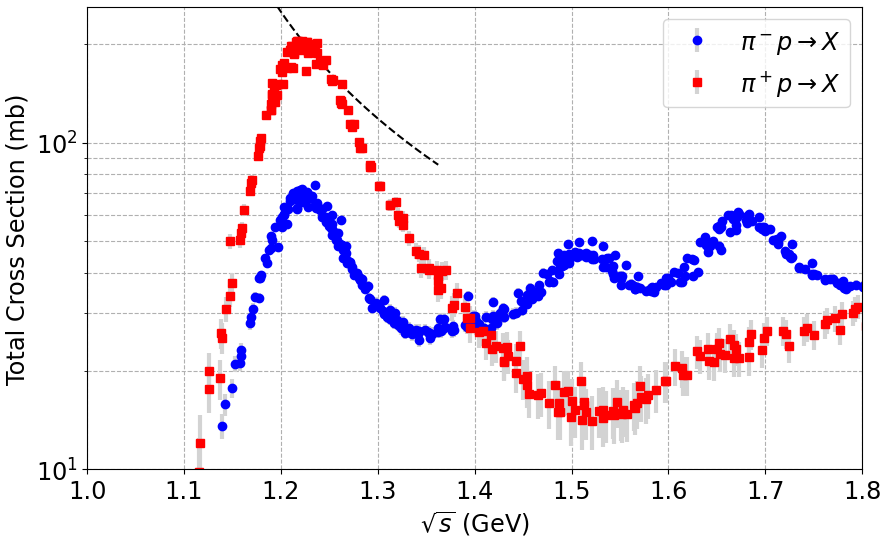
\includegraphics[width=0.8\textwidth]{pi_p_cross_section.png}
\end{center}


The cross section data should be taken from PDG:\\ 
\href{https://pdg.lbl.gov/2022/hadronic-xsections/hadron.html}{https://pdg.lbl.gov/2022/hadronic-xsections/hadron.html}.

%%%%%%%%%%%%%%%%%%%%%%%%%%%%%%%%%%%%%%%%%%%%%%%%%%%%%%%
%%%%%%%%%%%%%%%%%%%%%%%%%%%%%%%%%%%%%%%%%%%%%%%%%%%%%%%
\end{document}
